\documentclass[12pt]{article}
\usepackage[russian]{babel}
\usepackage[utf8x]{inputenc}
\usepackage{amssymb}
\usepackage{amsmath}
\usepackage{graphicx}
\usepackage{geometry}
\usepackage[colorinlistoftodos]{todonotes}
\usepackage{listings}
\usepackage[section]{placeins}
\begin{document}

\title{6. Спектральное оценивание при помощи коррелограммного метода}
\author{Андрей Валиков}
\date{}
\maketitle
																																																								\section{Вычисление спектральной плотности для гармонической функции}
																																																	
\[N = 2^{11}\]  

Гармоническая функция
\[y=A\sin(\omega_{1}Tn + \varphi)\]
	

\begin{lstlisting}
N = 2 ** 11
T = 2e-2
t = np.linspace(0, T, N)

A = 2
fi = 2.09
wi = 100

y = A * np.sin(wi * t + fi)

Y = np.fft.fft(y)
YY = Y * np.conj(Y) / N

plt.plot(t, YY)
plt.savefig('spectral_density.png')
plt.show()
\end{lstlisting}

Спектральная плотность гармонической функции
\begin{figure}[!htb]
\centering
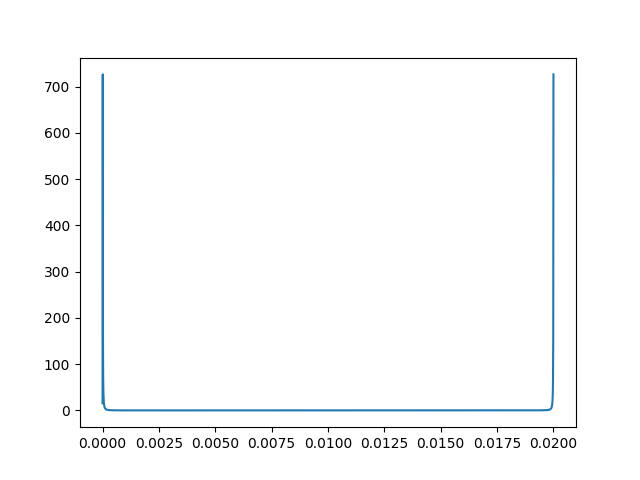
\includegraphics[scale=1.00]{spectral_density.png}
\caption{}
\label{}
\end{figure}


\section{Формирование последовательности}


\[f = \sin(\omega_1 Tt) + \cos(\omega_2 Tt)\]


\begin{lstlisting}
teta = np.arange(0, N, 1)
w1 = 81
w2 = 14
b = 5

x = np.sin(w1 * T * teta) + np.cos(w2 * T * teta)

r = b * np.random.rand(N)

y = x + (r - np.mean(r))

plt.plot(teta, x)
plt.show()

plt.plot(teta, r)
plt.show()

plt.plot(teta, y)
plt.show()
\end{lstlisting}


\begin{figure}[!htb]
\centering
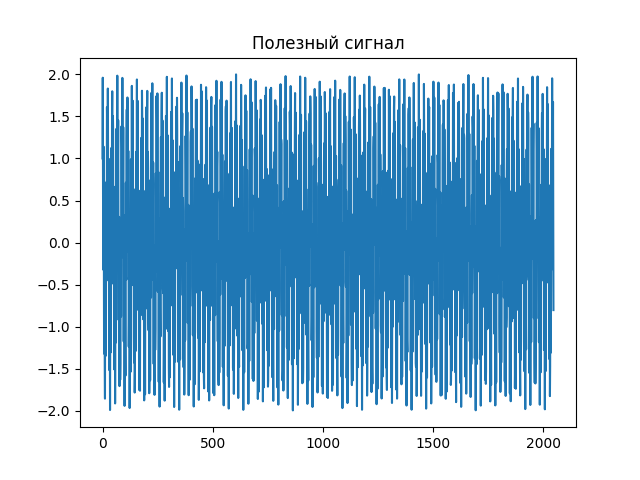
\includegraphics[scale=1.00]{good.png}
\caption{}
\label{}
\end{figure}

\begin{figure}[!htb]
\centering
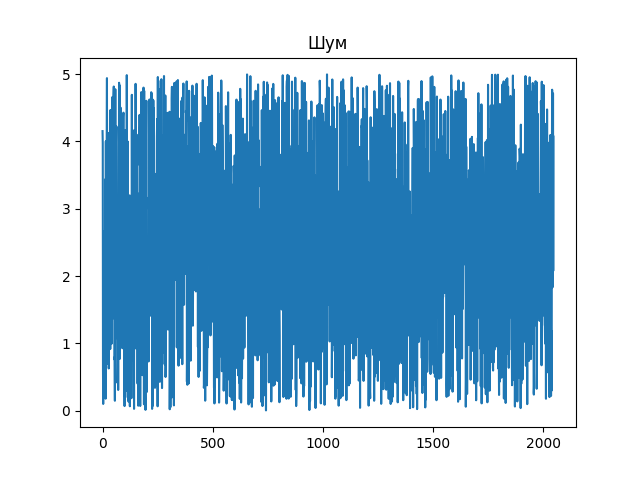
\includegraphics[scale=1.00]{bad.png}
\caption{}
\label{}
\end{figure}

\begin{figure}[!htb]
\centering
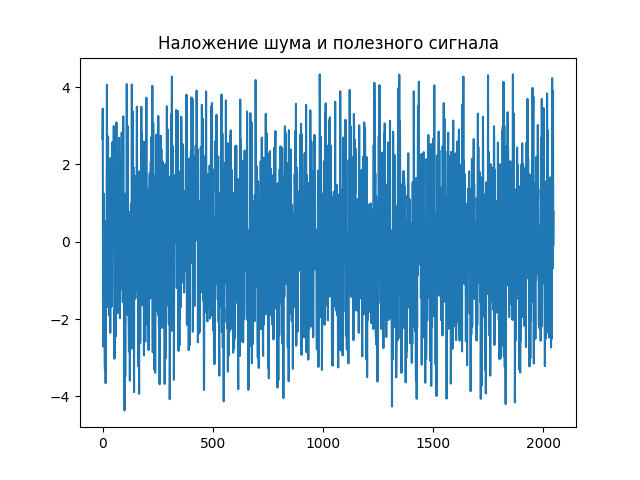
\includegraphics[scale=1.00]{ugly.png}
\caption{}
\label{}
\end{figure}


\section{Расчет оценки спектральной плотности коррелограммным методом с прямоугольным окном}




\begin{lstlisting}

#Corell function
r = np.zeros(int(len(y) / 10 - 1))
for i in range(len(r)):
  for j in range(N - i):
      r[i] += y[j] * y[j + i]
  r[i] /= len(y) - i

#Spectral density
w = np.linspace(0, np.pi / T, N)
y = np.zeros(len(w))
for n in range(len(w)):
  for m in range(len(r)):
      y[n] += r[m] * np.cos(w[n] * T * m)
  y[n] *= 2


plt.plot(w, y)
plt.show()

plt.plot(w, np.abs(y))
plt.show()
\end{lstlisting}


\begin{figure}[!htb]
\centering
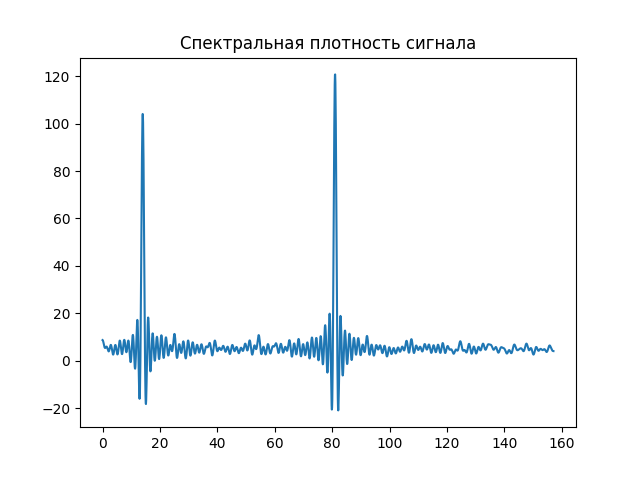
\includegraphics[scale=1.00]{sig_spectral_density.png}
\caption{}
\label{}
\end{figure}

\begin{figure}[!htb]
\centering
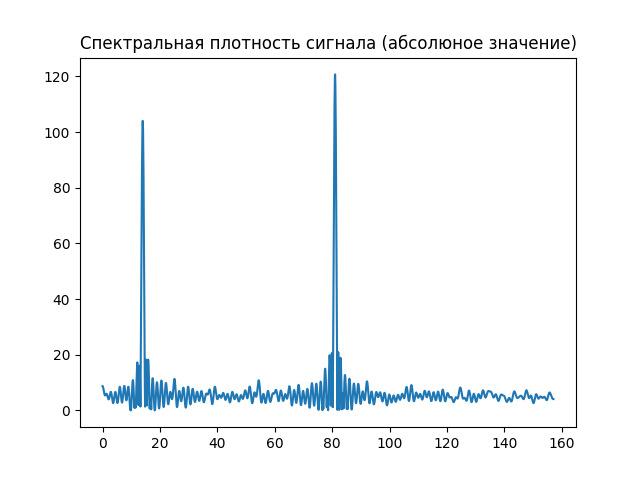
\includegraphics[scale=1.00]{sig_spectral_density_abs.png}
\caption{}
\label{}
\end{figure}



\section{Расчет оценки спектральной плотности по методу коррелограмм с использованием оконной функции}

\begin{lstlisting}

max_num = Search(y)

ww1 = np.pi * max_num[0] / (128 * T)
ww2 = np.pi * max_num[1] / (128 * T)

bartletta_window = np.zeros(len(r))
ht = np.arange(0, len(r), 1)

for i in range(len(ht)):
  if ht[i] >= 0 and ht[i] <= len(ht):
    bartletta_window[i] = .42 - .5 * np.cos(2 * np.pi * ht[i] / len(ht)) + .08 * np.cos(4 * np.pi * ht[i] / len(ht))

plt.plot(ht, bartletta_window)
plt.show()

y1 = np.zeros(len(w))
for n in range(len(w)):
  for m in range(len(r)):
    y1[n] += r[m] * bartletta_window[m] * np.cos(w[n] * T * m)
    y1[n] *= 2

plt.plot(w, y1)
plt.plot(w, np.abs(y1))
plt.show()

max_num = Search(y1)
ww1_1 = np.pi * max_num(0) / (128 * T)
ww2_2 = np.pi * max_num(1) / (128 * T)
\end{lstlisting}

\begin{figure}[!htb]
\centering
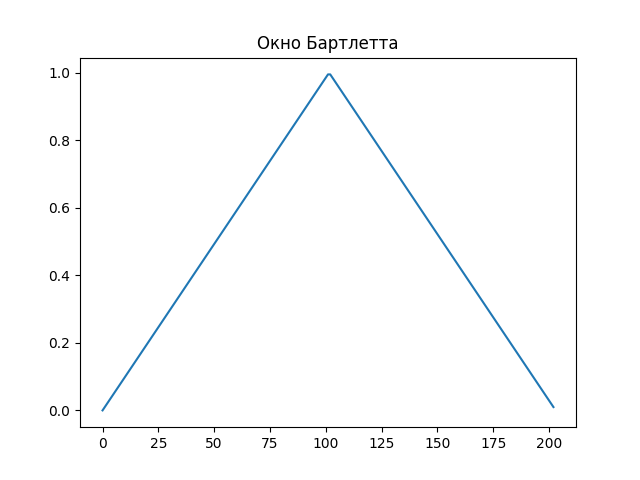
\includegraphics[scale=1.00]{bartletta_window.png}
\caption{}
\label{}
\end{figure}

\begin{figure}[!htb]
\centering
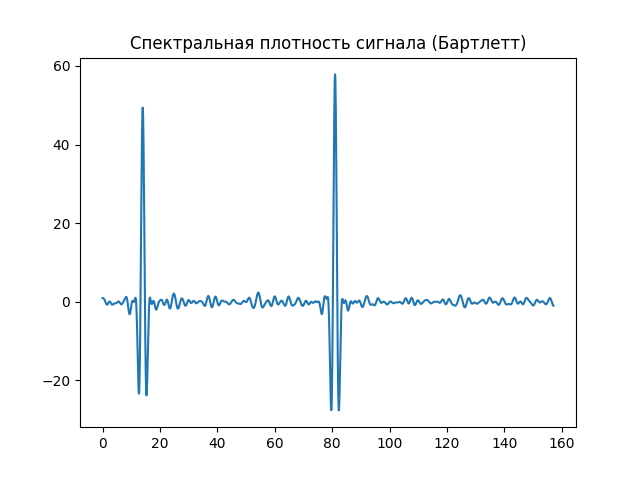
\includegraphics[scale=1.00]{sig_spectral_density_bart.png}
\caption{}
\label{}
\end{figure}

\begin{figure}[!htb]
\centering
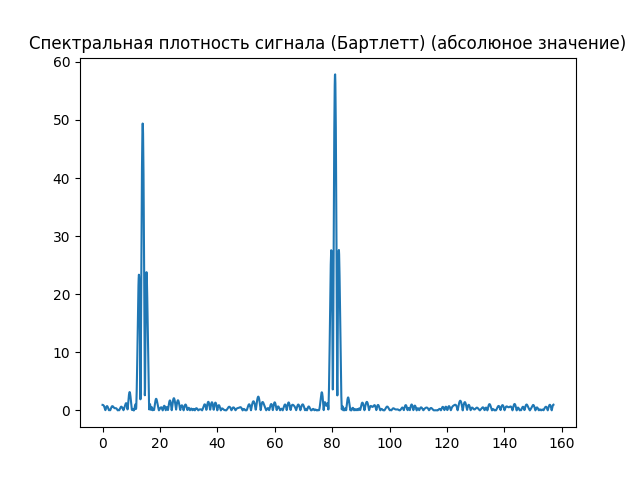
\includegraphics[scale=1.00]{sig_spectral_density_bart_abs.png}
\caption{}
\label{}
\end{figure}



\section{Вывод}
Изучен каррелограммный метод оценивания спектральной плотности на тестовой последовательности дискретных значений с наложенным случайным процессом. Была найдена корреляционная функция и её спектральная плотность по методу прямоугольно окна. Далее была выбрана оконная функция Барлетта и найдена уже её спектральная плотность.\\
В результате работы программы были получены следующие угловые частоты:\\
    • С использование прямоугольного окна\\
$\omega_{1}$ = 148.16\\
$\omega_{2}$ = 147.85\\
\\
    • С использование оконной функции Бартлетта\\
$\omega_{1bart}$ = 71\\
$\omega_{2bart}$ = 70.83\\

Графики спектральной плотности двух методов отличаются. Благодаря использованию оконной функции Бартлетта было убрано явление Гиббса, возникновение которого связано с использованием прямоугольного окна.

\end{document}